\documentclass[titlepage,10pt,a4paper]{jsbook}

\usepackage{textcomp}

\setcounter{tocdepth}{4}

\usepackage[round,colon,authoryear]{natbib}

\usepackage[dvipdfmx, hiresbb]{graphicx, xcolor}

\usepackage{grffile}

\usepackage[%
dvipdfm,%
pdfstartview={FitH -32768},%    描画領域の幅に合わせる
bookmarks=true,%                しおり付き
bookmarksnumbered=false,%        章や節の番号をふる
bookmarkstype=toc,%             目次情報のファイル.tocを参照
colorlinks=true,%              ハイパーリンクを色文字に
linkcolor=black,%       link の枠の色 black
citecolor=black,%       cite の枠の色 black
urlcolor=black,%        url の枠の色 black
pdftitle={生態学のためのメタバーコーディングとDNAバーコーディング:採集・分子実験編},%
pdfauthor={田辺晶史},
pdfkeywords={メタゲノム, 環境DNA}%
]{hyperref}
\usepackage{pxjahyper}

\usepackage{pxfonts}

\bibliographystyle{jecon}

\makeatletter
\def\maketitle{%
  \begin{center}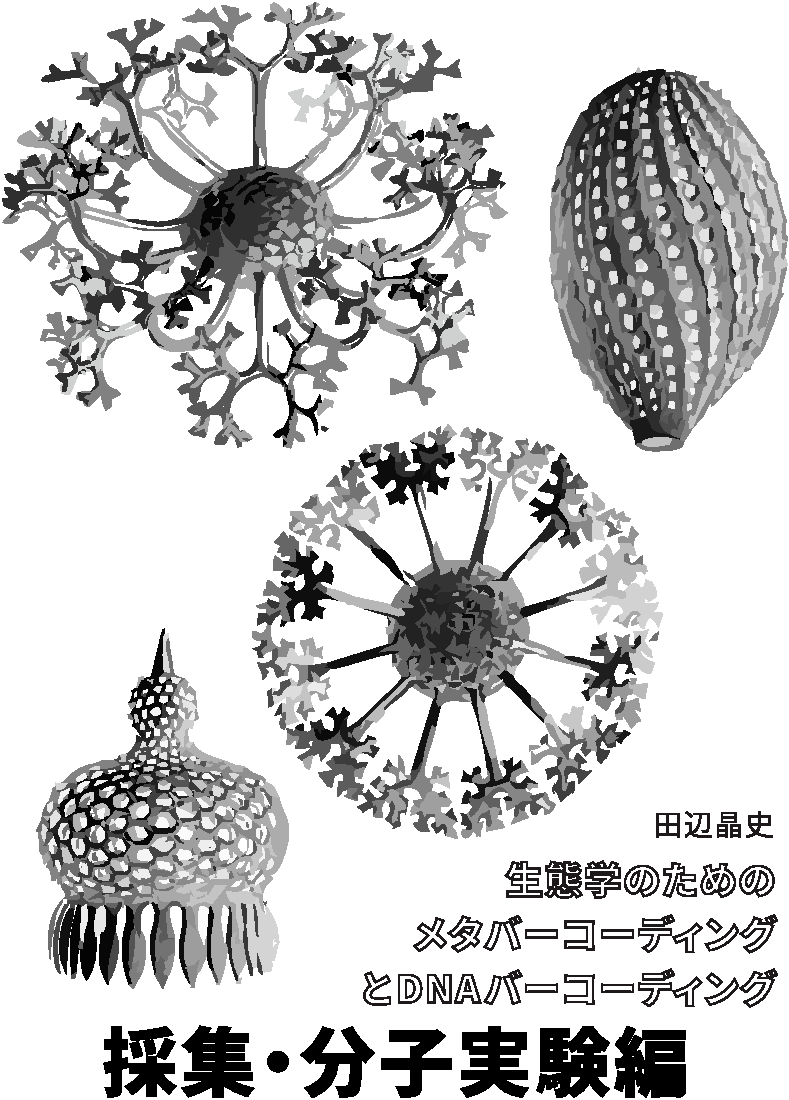
\includegraphics[pagebox=cropbox,clip]{metabarcodingtextbook1.ja.title.pdf}\end{center}%
  \cleardoublepage
  \begin{titlepage}%
    \let\footnotesize\small
    \let\footnoterule\relax
    \let\footnote\thanks
    \null\vfil
    \vskip 60\p@
    \begin{center}%
      {\LARGE \@title \par}%
      \vskip 3em%
      {\large
        \lineskip .75em
        \begin{tabular}[t]{c}%
          \@author
        \end{tabular}\par}%
      \vskip 1.5em
      {\large \@date \par}%
    \end{center}%
    \par
    \@thanks\vfil\null
  \end{titlepage}%
  \setcounter{footnote}{0}%
  \global\let\thanks\relax
  \global\let\maketitle\relax
  \global\let\@thanks\@empty
  \global\let\@author\@empty
  \global\let\@date\@empty
  \global\let\@title\@empty
  \global\let\title\relax
  \global\let\author\relax
  \global\let\date\relax
  \global\let\and\relax
}
\makeatother

\title{生態学のためのメタバーコーディングとDNAバーコーディング:採集・分子実験編}
\author{田辺晶史}
\date{\today}

%\renewcommand{\baselinestretch}{1.2}
\renewcommand{\prepartname}{第}
\renewcommand{\postpartname}{部}
\renewcommand{\prechaptername}{第}
\renewcommand{\postchaptername}{章}
\renewcommand{\presectionname}{}%  第
\renewcommand{\postsectionname}{}% 節
\renewcommand{\contentsname}{目次}
\renewcommand{\listfigurename}{図目次}
\renewcommand{\listtablename}{表目次}
\renewcommand{\refname}{引用文献}
\renewcommand{\bibname}{引用文献}
\renewcommand{\indexname}{索引}
\renewcommand{\figurename}{図}
\renewcommand{\tablename}{表}
\renewcommand{\appendixname}{付録}

\usepackage{float}
\usepackage{framed}
\definecolor{shadecolor}{gray}{0.9}
\newenvironment{content}{\begin{shaded}\vspace{-1em}\raggedright\ttfamily\footnotesize\setlength{\baselineskip}{1.4em}}{\end{shaded}\vspace{-1em}}
\newenvironment{pre}{\begin{leftbar}\raggedright\ttfamily\footnotesize\setlength{\baselineskip}{1.4em}}{\end{leftbar}\vspace{-1em}}
\newenvironment{cmd}{\begin{oframed}\raggedright\ttfamily\footnotesize\setlength{\baselineskip}{1.4em}}{\end{oframed}\vspace{-1em}}

\setlength{\textwidth}{\fullwidth}
\setlength{\evensidemargin}{\oddsidemargin}
\addtolength{\evensidemargin}{-2.5 true mm}
\addtolength{\oddsidemargin}{2.5 true mm}

\makeatletter
\renewcommand{\chapter}{%
  \if@openright\cleardoublepage\else\clearpage\fi
  \global\@topnum\z@
  \secdef\@chapter\@schapter}
\makeatother

\begin{document}
\thispagestyle{empty}
\maketitle
\cleardoublepage
\pagenumbering{roman}
\tableofcontents
\cleardoublepage
\setlength{\parindent}{0em}
\setlength{\parskip}{1em plus 0.2em}
\parindent=0em
\parskip=1em plus 0.2em
\pagenumbering{arabic}

\chapter*{はじめに}
\addcontentsline{toc}{chapter}{はじめに}

本書はクリエイティブ・コモンズの表示-継承 4.0 国際ライセンスの下で配布します。
このライセンスの下では、原著作者の明示を行う限り、利用者は自由に本書を複製・頒布・展示することができます。
また、原著作者の明示と本ライセンスまたは互換性のあるライセンスの適用を行う限り、本書を改変した二次著作物の作成・配布も自由に行うことができます。
詳しい使用許諾条件を見るには\\
\href{https://creativecommons.org/licenses/by-sa/4.0/}{https://creativecommons.org/licenses/by-sa/4.0/}\\
をチェックするか、クリエイティブ・コモンズに郵便にてお問い合わせください。
住所は Creative Commons, PO Box 1866, Mountain View, CA 94042, USA です。

本書が皆さんの役に立つことができましたら幸いです。
この機会を与えて下さった京都大学生態学研究センターの東樹宏和博士、水産研究・教育機構中央水産研究所の長井敏博士、龍谷大学の山中裕樹博士と、本書をお読みの皆さんに感謝します。

\chapter{環境DNA・メタゲノムDNAの採集方法}

ここでは、水からの環境DNA採集、および水、土壌、糞などからのメタゲノムDNAの採集方法について解説します。
DNA抽出用の個体や組織の採集方法はここでは取り扱いません。
なお、環境DNAとメタゲノムDNAは識別困難ですが、ここでは、環境DNAを「生物個体から排出されたDNA」、メタゲノムDNAを「生物個体から排出されていないDNA」ということにします。
したがって、水中の魚類や甲殻類、水生昆虫、水生植物のDNAは環境DNAであり、微生物のDNAはメタゲノムDNAであることが多いでしょう(ただし、区別できないだけで微生物の環境DNAも含まれているでしょう)。
また、未消化物に含まれる被食者や本人のDNAはどちらにするか難しいところですが、とりあえずメタゲノムDNAということにしておきます。

\section{サンプリングデザイン}

採集地点・時間をどのように配置するかは研究の内容に直結する重要な課題です。
ここで研究目的の達成の可否が決まると言っても過言ではありません。
そのためには、研究目的の明確化と予備調査が必須です。

例えば、ため池ごとの魚類相と環境条件(池の大きさ、深さ、水質、地質、高度、緯度経度など)との関連性を解明したいが、ため池の中での微細な違いには興味がないケースでは、ため池がよほど小さくない限り、ため池内の数地点から水を採集し、混合して濾過採集することになります。
ため池が非常に小さい場合や、ため池内の水が十分に混合されていたり、対象となるため池があまりに多い場合は、1地点だけでため池を代表させることもあるでしょう。
もちろん、余裕があるならため池内の数地点のサンプルを全て別々にして、その気になればため池内の微細な違いをも解析可能にしておくことも悪くありませんが、後述するサンプルレプリケートを複数用意することを考えると、大きな労力が必要となりますので、人手を十分考慮する必要があります。
また、その場合はため池内の数地点のサンプル間でDNA抽出効率・PCR増幅効率などに大きな違いが生じることがないようにしなくてはなりません(違う場合は環境条件の影響と言えなくなってしまう)。

別のケースとして、森林の土壌を分析して、微生物叢と植物相の関連性を解明したい場合を考えましょう。
この場合、1地点を広くかつ深く取り、その範囲の土壌を混合して採集するか、その範囲の土壌からいくつかのサブサンプルを採集して混合するのがよいでしょう。
土壌では、少し離れただけで全く異なる微生物叢を示すので、ある場の植物相と対応する微生物叢を完全な1点では代表することができません。
そのため、植物相と対応する範囲の数地点のサブサンプルをプールすることで代表させます。

以上のように、「DNAの拡散する範囲」と「そのサンプルで代表させたい範囲」を考慮して、前者の範囲の方が広くなるようにサンプリングデザインを行う必要があります。
後者の範囲の方が広くなってしまう場合、研究の目的とする議論が行えなくなることがあります。
ただ、後者の範囲の方が広くなる場合でも、サンプルが大量にあるのであれば、「本来の生物相」と「サンプルの生物相」との乖離に何らかの偏りがない限りは目的の議論ができる場合もあるでしょう。

\section{テクニカルレプリケートとネガティブコントロール}

1サンプルを1レプリケートで採集した場合、DNA抽出効率やPCR増幅効率のばらつきの影響を受けます。
また、レアな種のゲノムDNAや低濃度の環境DNAはサンプルに入ったり入らなかったりすることもあり得ます。
そこで、可能であれば複数(3以上ならなお良い)のレプリケートを1サンプル中に用意することが望ましくなります。
このようにすることで、各サンプルごとに種の「発見率」を推定することができます。
例えば、1サンプルが10レプリケート含んでいるとき、x軸をレプリケート数、y軸を合計種数とする折れ線グラフを描くことを想像してください。
10レプリケートからx軸のレプリケート数だけ無作為抽出して合計種数を算出してy軸の合計種数を計算します。
このとき、折れ線が傾きゼロの直線なら1レプリケートでも発見率は100\%と考えられ、x=1では傾きゼロではなくとも、x=10では傾きゼロになっているなら10レプリケート合計すれば飽和している=発見率100\%ということになります。
しかし、x=10でも線が傾いているようであれば、発見率は100\%ではなく、いくらか取りこぼしがあることがわかります。
発見率が100\%であることが理想ですが、必ずしもそうである必要はありません。
重要なのは、発見率が推定できることです。

\section{水からの濾過採集方法}

\subsection{濾過フィルターと濾過方法と固定方法の選定}

\subsection{濾過関連機材の塩素漂白の方法}

\subsubsection{必要な機材}
\begin{itemize}
\item 水道
\item 蛇口に適合するシリコンチューブ (厚さは任意) 1本
\item 漂白剤抜き器 (作成方法は付録\ref{makingdebleachcontainer}を参照) 1個
\item 漂白対象物が入る大きさのタッパーやビーカー 1個
\item 防水作業着 1着
\end{itemize}

\subsubsection{必要な消耗品}
\begin{itemize}
\item 花王 ハイターE (界面活性剤なしの塩素系漂白剤。次亜塩素酸ナトリウム6\%) 適量
\item 使い捨てゴム手袋 1双
\item SPW 適量
\end{itemize}

\subsubsection{作業手順}
\begin{enumerate}
\item 漂白対象物が入る大きさのタッパーやビーカーに漂白対象物を入れる
\item 漂白対象物が浸かるように水道水を注ぐ
\item 水道水の5~10\%量のハイターEを入れてかき混ぜる
\item 漂白対象物が水に浮く場合、同サイズのタッパーやビーカーを重ねて重しを入れて押さえつける (これができるような形状のタッパーやビーカーを使用する)
\item 時々ゆすりながら30分以上、できれば1時間以上浸ける (ただし浸け過ぎに注意)
\item 漂白液を捨てて漂白対象物を漂白剤抜き器に移す
\item 漂白剤抜き器のホースニップルと水道の蛇口をシリコンチューブで接続する
\item 水道水を上限まで注いで捨てる
\item 漂白対象物が
\begin{enumerate}
\item 水に浮く場合、水道水を勢いよく流しっぱなしにして30分以上放置して水を捨てる (水の勢いで漂白対象物が動くようにする)
\item 水に沈む場合、水道水を上限まで注いで捨てることを更に2回繰り返す
\end{enumerate}
\item 漂白対象物が入る大きさのタッパーやビーカーに漂白対象物を移す
\item SPWを漂白対象物が浸かるように注いですすいで捨てる
\item 乾燥が必要な場合はアルミホイルに包んで常温~60℃で乾燥する (60℃にする前に一度200℃以上で庫内を滅菌してから60℃に下げること)
\end{enumerate}

なお、漂白剤抜き器を漂白対象物が入る大きさのタッパーとして使用しても問題ありません。
また、漂白対象物が小さい場合、全ての作業をタッパーやビーカーで行っても構いません。
フィルターホルダーはパッキンやアダプタを外して分解し、個別に漂白を行い、漂白後に組み立てます。

\subsection{吸引濾過装置を用いた水からの微生物メタゲノムDNA・環境DNAの濾過採集方法}

\subsubsection{必要な機材}
\begin{itemize}
\item DC12Vのシガーソケット搭載車 または ACアダプタ 1個
\item 車載用吸引ポンプユニット (作成方法は付録\ref{makingpumpunit}を参照) 1個
\item 吸引濾過装置 (作成方法は付録\ref{makingfilteringunit}を参照) 1個
\item toolsisland 手動式オイルチェンジャー または メルテック オイルチェンジャー OC-060 1個
\item アズワン 穴付きシリコン栓 8号 (1-7650-01) の両方の穴に 光 ステンレス丸パイプ 外径6mm を適当な長さに切断して挿したもの (長さを不揃いにすること) 1個
\item アズワン シリコンチューブ 内径5mm 外径6mm 長さ1m (6-586-19-01) 1本
\item アズワン シリコンチューブ 内径5mm 外径6mm 長さ1m (6-586-19-01) を切断して途中に Whatman VACU-GUARD (6722-5000) を挟んだもの 1本
\item モンキーレンチ 1本 (ディスクフィルター使用時のみ)
\item サンダイヤ デッキ型ピンセット 125mm (アズワン品番 6-531-12) 1本 (ディスクフィルター使用時のみ)
\item ハサミ 1本
\item ライター 1本
\item ゼブラ マッキープロ細字 特殊用途DX 1本 (色の薄いハズレ個体がよくあるので予め確認しておく)
\item 三菱アルミニウム 三菱ホイル タフ 30cm×50m 1本
\item ロゴス ハイパー氷点下クーラーM No.81670070 1個
\item ロゴス 倍速凍結・氷点下パックXL No.81660640 2個以上 (必ず氷点下を維持できる保冷剤を使用すること)
\end{itemize}

\subsubsection{必要な消耗品}
\begin{itemize}
\item 以下のいずれかの濾過フィルターユニット 1個/1サンプル
\begin{itemize}
\item アズワン FH-PP47 (3-6736-01) または ADVANTEC PP-47 に47mmディスクフィルターを詰めたもの (漂白で再利用可)
\item Millipore Sterivex-HV 0.45{\textmu}m PVDF SVHV010RS
\item Millipore Sterivex-GV 0.22{\textmu}m PVDF SVGV010RS
\item Millipore Sterivex-GP 0.22{\textmu}m PES SVGP01050
\end{itemize}
\item フィルターユニットに適合するアダプタ (作成方法は付録\ref{makingfilteradapter}を参照) 1個/1サンプル (漂白で再利用可)
\item 以下のいずれかのプラスチックバッグ 1個/1サンプル
\begin{itemize}
\item カウパック 夢パック 100mL DP16-TN0100
\item カウパック 夢パック 200mL DP16-TN0200
\item カウパック 夢パック 300mL DP16-TN0300
\item カウパック 夢パック 500mL DP16-TN0500
\item カウパック 夢パック 1000mL DP16-TN1000
\end{itemize}
\item 以下のいずれかの使い捨てビーカー 1個/1サンプル
\begin{itemize}
\item 大塚刷毛製造 補修用カップ 容器のみ 400mL 3221110400
\item 大塚刷毛製造 補修用カップ 容器のみ 600mL 3221110600
\item 大塚刷毛製造 補修用カップ 容器のみ 800mL 3221110800
\item ビッグ 調色ミキシングカップ 1000mL MK11L
\end{itemize}
\item セイニチ ユニパック C-4 1枚/1サンプル
\item 使い捨てポリ手袋 2双/1サンプル
\end{itemize}

\subsubsection{作業手順}
\begin{enumerate}
\item 車載用吸引ポンプユニットのバルブは開放しておく
\item 吸引濾過装置のバルブは全て閉じておく
\item シガーソケットに車載用吸引ポンプユニットの電源を接続する
\item 車載用吸引ポンプユニットのホースニップルにVACU-GUARDを取り付けたシリコンチューブ経由で穴付きシリコン栓の短い方のステンレスパイプを接続する
\item 穴付きシリコン栓を手動式オイルチェンジャーのタンクに挿す
\item 穴付きシリコン栓の長い方のステンレスパイプにもう一つのシリコンチューブ経由で吸引濾過装置を接続する
\item ポリ手袋を着ける
\item 使い捨てビーカーで必要量の水試料を量り取り、プラスチックバッグに入れる
\item 濾過フィルターユニットにアダプタを取り付ける (ディスクフィルター使用の場合はモンキーレンチでしっかり締め付ける)
\item アダプタの反対側に水試料の入ったプラスチックバッグを取り付ける (アダプタの接着面に力がかからないように注意すること)
\item プラスチックバッグ+濾過フィルターユニットを濾過フィルターユニットが下になるように吸引濾過装置に取り付け、リピートバンドを締める
\item 吸引濾過装置のバルブ(プラスチックバッグからタンクの経路上のもの)を開ける
\item 車載用吸引ポンプユニットの電源を入れ、水試料を吸引する
\item 水試料吸引開始後、プラスチックバッグ上端にハサミで切り込みを入れる (ハサミが水試料に接さないように注意。必要に応じてハサミをライターで火炎滅菌する)
\item 水試料の吸引が終わったら、吸引濾過装置の濾過フィルターユニット直下のバルブを閉じる
\item リピートバンドを緩めてプラスチックバッグ+濾過フィルターユニットを吸引濾過装置から外す
\item 濾過フィルターユニットからプラスチックバッグを取り外して捨てる (アダプタは残す)
\item 濾過フィルターユニットを再度吸引濾過装置に取り付け、濾過フィルターユニット直下のバルブを開けて濾過フィルターユニット内の残留水を吸引する (濾過フィルターユニットを独楽のように回して吸引する)
\item アルミホイルを適当な長さで切って折り目を付けておく
\item 吸引濾過装置の濾過フィルターユニット直下のバルブを閉じて車載用吸引ポンプユニットの電源を切る
\item 濾過フィルターユニットを吸引濾過装置から外す
\item ポリ手袋を交換する
\item 濾過フィルターユニットが
\begin{enumerate}
\item フィルターホルダー+ディスクフィルターの場合、アダプタはそのままにして分解し、フィルターを分解してライターで火炎滅菌したピンセットで二つ折りにしてアルミホイルで包んでマッキープロでサンプル情報を記述し、ユニパックに入れ、クーラーバッグに保冷剤で挟まれるように入れる
\item Sterivexの場合、アダプタを外してアルミホイルで包んでから、マッキープロでサンプル情報を記述したユニパックに入れ、クーラーバッグに保冷剤で挟まれるように入れる
\end{enumerate}
\item ポリ手袋を外して捨てる
\item 吸引濾過装置の両側下部バルブを開放する (吸引濾過装置内の残留水がタンクに吸い込まれる)
\item 手動式オイルチェンジャーのタンクからシリコン栓を外し、中の廃液を捨てる
\end{enumerate}

なお、アズワンFH-PP47およびADVANTEC PP-47のパッキンが劣化した場合、シリコンゴムかフッ素ゴム製のAS568-030型およびAS568-033型の品に交換することができます。
ここではSterivexをすぐに冷凍する方法を示しましたが、中にRNAlaterを注入して両端にキャップ(テルモ テルフュージョン三方活栓キャップ密栓用 XX-WS01K* および コクゴ 点眼キャップ赤3φ 101-5210102)を付けて冷凍・冷蔵・常温保管する方法もあります。
海外などで冷凍手段が確保できない場合にはこの方法を用いることになります。

\subsection{シリンジを用いた水からのメタゲノムDNA・環境DNAの濾過採集方法}

\subsubsection{必要な機材}
\begin{itemize}
\item タジマ コンボイVS CNV-VS
\item ゼブラ マッキープロ細字 特殊用途DX 1本 (色の薄いハズレ個体がよくあるので予め確認しておく)
\item 三菱アルミニウム 三菱ホイル タフ 30cm×50m 1本
\item ロゴス ハイパー氷点下クーラーM No.81670070 1個
\item ロゴス 倍速凍結・氷点下パックXL No.81660640 2個以上 (必ず氷点下を維持できる保冷剤を使用すること)
\end{itemize}

\subsubsection{必要な消耗品}
\begin{itemize}
\item テルモ テルモシリンジ ロック付 50mL SS-50LZ 1本/1サンプル
\item 大阪魂 丸ワッシャー 特寸 鉄/生地 M17×外径50mm×厚さ3.2mm 1枚/1サンプル (乾熱滅菌で再利用可)
\item 以下のいずれかの濾過フィルターユニット 1個/1サンプル
\begin{itemize}
\item Millipore Sterivex-HV 0.45{\textmu}m PVDF SVHV010RS
\item Millipore Sterivex-GV 0.22{\textmu}m PVDF SVGV010RS
\item Millipore Sterivex-GP 0.22{\textmu}m PES SVGP01050
\end{itemize}
\item 以下のいずれかの使い捨てビーカー 1個/1サンプル
\begin{itemize}
\item 大塚刷毛製造 補修用カップ 容器のみ 400mL 3221110400
\item 大塚刷毛製造 補修用カップ 容器のみ 600mL 3221110600
\item 大塚刷毛製造 補修用カップ 容器のみ 800mL 3221110800
\item ビッグ 調色ミキシングカップ 1000mL MK11L
\end{itemize}
\item セイニチ ユニパック C-4 1枚/1サンプル
\item 使い捨てポリ手袋 1双/1サンプル
\end{itemize}

\subsubsection{作業手順}
\begin{enumerate}
\item ポリ手袋を着ける
\item 使い捨てビーカーで必要量の水試料を量り取る
\item シリンジにビーカーから水試料50mLを吸い取る (水に浸かるシリンジ先端3cm程度は触れないようにする)
\item シリンジのルアーロック部にSterivexを取り付けてワッシャーに通す
\item Sterivexが先端から突き出すようにコーキングガンにセットする
\item コーキングガンの引き金を引いて加圧濾過する
\item シリンジ+Sterivexをコーキングガンから外す
\item Sterivexとシリンジを分離する
\item 必要量に達するまで3に戻って繰り返す
\item 必要な水量の濾過が終わったら、シリンジに空気をめいっぱい吸引する
\item シリンジのルアーロック部にSterivexを取り付けてワッシャーに通す
\item Sterivexが先端から突き出すようにコーキングガンにセットする
\item Sterivexが下になるように垂直に立ててコーキングガンの引き金を引き、できるだけSterivex内の水を抜く
\item シリンジ+Sterivexをコーキングガンから外す
\item Sterivexとシリンジを分離する
\item Sterivexをアルミホイルで包んでから、マッキープロでサンプル情報を記述したユニパックに入れ、クーラーバッグに保冷剤で挟まれるように入れる
\item ポリ手袋を外して捨てる
\end{enumerate}

ここではSterivexをすぐに冷凍する方法を示しましたが、中にRNAlaterを注入して両端にキャップ(テルモ テルフュージョン三方活栓キャップ密栓用 XX-WS01K* および コクゴ 点眼キャップ赤3φ 101-5210102)を付けて冷凍・冷蔵・常温保管する方法もあります。
海外などで冷凍手段が確保できない場合にはこの方法を用いることになります。

\chapter{DNA抽出・ライブラリ調製・シーケンシング}

\section{機材・試薬の滅菌とDNA分解によるコンタミネーションの防止}

\section{テクニカルレプリケートとネガティブコントロール}

\section{DNA抽出}

\subsection{47mmグラスファイバーフィルターからのDNA抽出プロトコル}

\subsubsection{必要な機材}
\begin{itemize}
\item 
\end{itemize}

\subsubsection{必要な試薬・消耗品}
\begin{itemize}
\item 
\end{itemize}

\subsubsection{作業手順}
\begin{enumerate}
\item 
\end{enumerate}

\subsection{47mm非グラスファイバーフィルターからのDNA抽出プロトコル}

\subsubsection{必要な機材}
\begin{itemize}
\item 
\end{itemize}

\subsubsection{必要な試薬・消耗品}
\begin{itemize}
\item 
\end{itemize}

\subsubsection{作業手順}
\begin{enumerate}
\item 
\end{enumerate}

\subsection{ステリべクスからのDNA抽出プロトコル}

\subsubsection{必要な機材}
\begin{itemize}
\item 
\end{itemize}

\subsubsection{必要な試薬・消耗品}
\begin{itemize}
\item 
\end{itemize}

\subsubsection{作業手順}
\begin{enumerate}
\item 
\end{enumerate}

\subsection{磁気ビーズを用いたDNAの精製プロトコル}

\subsubsection{必要な機材}
\begin{itemize}
\item 
\end{itemize}

\subsubsection{必要な試薬・消耗品}
\begin{itemize}
\item 
\end{itemize}

\subsubsection{作業手順}
\begin{enumerate}
\item 
\end{enumerate}

\section{ライブラリ調製}

\subsubsection{必要な機材}
\begin{itemize}
\item 
\end{itemize}

\subsubsection{必要な試薬・消耗品}
\begin{itemize}
\item 
\end{itemize}

\subsubsection{作業手順}
\begin{enumerate}
\item 
\end{enumerate}

\subsection{プライマーの設計と発注の方法}

\subsubsection{必要な機材}
\begin{itemize}
\item 
\end{itemize}

\subsubsection{必要な試薬・消耗品}
\begin{itemize}
\item 
\end{itemize}

\subsubsection{作業手順}
\begin{enumerate}
\item 
\end{enumerate}

\subsection{ユニバーサルプライマーを用いたPCRのプロトコル(泳動用)}

\subsubsection{必要な機材}
\begin{itemize}
\item 
\end{itemize}

\subsubsection{必要な試薬・消耗品}
\begin{itemize}
\item 
\end{itemize}

\subsubsection{作業手順}
\begin{enumerate}
\item 
\end{enumerate}

\subsection{アガロースゲル電気泳動のプロトコル}

\subsubsection{必要な機材}
\begin{itemize}
\item 
\end{itemize}

\subsubsection{必要な試薬・消耗品}
\begin{itemize}
\item 
\end{itemize}

\subsubsection{作業手順}
\begin{enumerate}
\item 
\end{enumerate}

\subsection{ユニバーサルプライマーを用いたPCRのプロトコル(本番用)}

\subsubsection{必要な機材}
\begin{itemize}
\item 
\end{itemize}

\subsubsection{必要な試薬・消耗品}
\begin{itemize}
\item 
\end{itemize}

\subsubsection{作業手順}
\begin{enumerate}
\item 
\end{enumerate}

\subsection{磁気ビーズを用いたPCR産物の精製プロトコル}

\subsubsection{必要な機材}
\begin{itemize}
\item 
\end{itemize}

\subsubsection{必要な試薬・消耗品}
\begin{itemize}
\item 
\end{itemize}

\subsubsection{作業手順}
\begin{enumerate}
\item 
\end{enumerate}

\subsection{Exonuclease Iを用いたPCR産物の精製プロトコル}

\subsubsection{必要な機材}
\begin{itemize}
\item 
\end{itemize}

\subsubsection{必要な試薬・消耗品}
\begin{itemize}
\item 
\end{itemize}

\subsubsection{作業手順}
\begin{enumerate}
\item 
\end{enumerate}

\subsection{アダプターを付加するPCRのプロトコル}

\subsubsection{必要な機材}
\begin{itemize}
\item 
\end{itemize}

\subsubsection{必要な試薬・消耗品}
\begin{itemize}
\item 
\end{itemize}

\subsubsection{作業手順}
\begin{enumerate}
\item 
\end{enumerate}

\subsection{インデックスとP5・P7アダプターを付加するPCRのプロトコル}

\subsubsection{必要な機材}
\begin{itemize}
\item 
\end{itemize}

\subsubsection{必要な試薬・消耗品}
\begin{itemize}
\item 
\end{itemize}

\subsubsection{作業手順}
\begin{enumerate}
\item 
\end{enumerate}

\subsection{磁気ビーズを用いたPCR産物の濃度均一化}

\subsubsection{必要な機材}
\begin{itemize}
\item 
\end{itemize}

\subsubsection{必要な試薬・消耗品}
\begin{itemize}
\item 
\end{itemize}

\subsubsection{作業手順}
\begin{enumerate}
\item 
\end{enumerate}

\subsection{E-Gel SizeSelectによるサイズ選択}

\subsubsection{必要な機材}
\begin{itemize}
\item 
\end{itemize}

\subsubsection{必要な試薬・消耗品}
\begin{itemize}
\item 
\end{itemize}

\subsubsection{作業手順}
\begin{enumerate}
\item 
\end{enumerate}

\section{ライブラリのクオリティチェック}

\subsection{Qubitによる濃度測定と希釈}

\subsubsection{必要な機材}
\begin{itemize}
\item 
\end{itemize}

\subsubsection{必要な試薬・消耗品}
\begin{itemize}
\item 
\end{itemize}

\subsubsection{作業手順}
\begin{enumerate}
\item 
\end{enumerate}

\subsection{Bioanalyzerによる電気泳動}

\subsubsection{必要な機材}
\begin{itemize}
\item 
\end{itemize}

\subsubsection{必要な試薬・消耗品}
\begin{itemize}
\item 
\end{itemize}

\subsubsection{作業手順}
\begin{enumerate}
\item 
\end{enumerate}

\section{MiSeqによるシーケンス}

\subsubsection{必要な機材}
\begin{itemize}
\item 
\end{itemize}

\subsubsection{必要な試薬・消耗品}
\begin{itemize}
\item 
\end{itemize}

\subsubsection{作業手順}
\begin{enumerate}
\item 
\end{enumerate}

\bibliography{metabarcodingtextbook1.ja}
\addcontentsline{toc}{chapter}{引用文献}

\appendix

\chapter{DNA採集関連機材の自作}

\section{漂白剤抜き器の作成}\label{makingdebleachcontainer}

\subsubsection{必要な機材}
\begin{itemize}
\item 
\end{itemize}

\subsubsection{必要な部材}
\begin{itemize}
\item 
\end{itemize}

\subsubsection{作業手順}
\begin{enumerate}
\item 
\end{enumerate}

\section{車載用吸引ポンプユニットの作成}\label{makingpumpunit}

\subsubsection{必要な機材}
\begin{itemize}
\item 
\end{itemize}

\subsubsection{必要な部材}
\begin{itemize}
\item 
\end{itemize}

\subsubsection{作業手順}
\begin{enumerate}
\item 
\end{enumerate}

\section{吸引濾過装置の作成}\label{makingfilteringunit}

\subsubsection{必要な機材}
\begin{itemize}
\item 
\end{itemize}

\subsubsection{必要な部材}
\begin{itemize}
\item 
\end{itemize}

\subsubsection{作業手順}
\begin{enumerate}
\item 
\end{enumerate}

\chapter{試薬の調製}

\section{DNA・RNA固定液の調製}

\subsubsection{必要な機材}
\begin{itemize}
\item 
\end{itemize}

\subsubsection{必要な試薬・消耗品}
\begin{itemize}
\item 
\end{itemize}

\subsubsection{作業手順}
\begin{enumerate}
\item 
\end{enumerate}

\section{DNA抽出用試薬の調製}

\subsection{Insect Lysis Buffer}

\subsubsection{必要な機材}
\begin{itemize}
\item 
\end{itemize}

\subsubsection{必要な試薬・消耗品}
\begin{itemize}
\item 
\end{itemize}

\subsubsection{作業手順}
\begin{enumerate}
\item 
\end{enumerate}

\subsection{Column Binding Buffer}

\subsubsection{必要な機材}
\begin{itemize}
\item 
\end{itemize}

\subsubsection{必要な試薬・消耗品}
\begin{itemize}
\item 
\end{itemize}

\subsubsection{作業手順}
\begin{enumerate}
\item 
\end{enumerate}

\subsection{Wash Buffer}

\subsubsection{必要な機材}
\begin{itemize}
\item 
\end{itemize}

\subsubsection{必要な試薬・消耗品}
\begin{itemize}
\item 
\end{itemize}

\subsubsection{作業手順}
\begin{enumerate}
\item 
\end{enumerate}

\section{PCR産物精製用磁気ビーズ液の調製}

\subsubsection{必要な機材}
\begin{itemize}
\item 
\end{itemize}

\subsubsection{必要な試薬・消耗品}
\begin{itemize}
\item 
\end{itemize}

\subsubsection{作業手順}
\begin{enumerate}
\item 
\end{enumerate}

\section{PCR産物濃度均一化用磁気ビーズ液の調製}

\subsubsection{必要な機材}
\begin{itemize}
\item 
\end{itemize}

\subsubsection{必要な試薬・消耗品}
\begin{itemize}
\item 
\end{itemize}

\subsubsection{作業手順}
\begin{enumerate}
\item 
\end{enumerate}

\end{document}
